\chapter{Numerical Analysis of IFB-HSB hybrid Connection}
\label{ch5}

%%%%%%%%%%%%%%%%%%%%%%%%%%%%%%%%%%%%%%%
% IMPORTANT
\begin{spacing}{1.25} %THESE FOUR
\minitoc % LINES MUST APPEAR IN
\end{spacing} % EVERY
\onehalfspacing % CHAPTER
% COPY THEM IN ANY NEW CHAPTER
%%%%%%%%%%%%%%%%%%%%%%%%%%%%%%%%%%%%%%%

\kant[1-2]


\section{Validation of FE model}

The modeling methods of  the original R12-O case in this analysis refer to the modeling method used in previous research \cite{Peng2013}, and the same analysis results were obtained.

We also referred to previously published experimental data \cite{peng2010} from other analyses to verify the modeling methods used in this study. The experimental setup is illustrated in Fig.\ref{fig-testset}, and the result of analysis and experiment is shown in Fig.\ref{fig-validloadrd}. The relative displacement taken from a distance of 10 mm from the inner end of the plate forms the reference for this experiment.

The analysis results were almost identical to the test results. Because the analysis used the penalty method to model contact and the static friction coefficient and isotropic Coulomb friction method to model friction, after the slip, the analysis would not be similar to the experiment in which the slip behavior was changed to kinetic friction and load reduction occurred. Therefore, the curve shape after the slip occurred, and the analysis and experimental results deviated. Therefore, the modeling methods used in this analysis can be considered valid.

For the hybrid joint, although the theoretically calculated value is the same as the analysis result, the verification of the mechanical behavior and failure mode of the hybrid joint will be conducted in a future study.

\begin{figure}
    \centering
    \begin{subfigure}[t]{0.4\textwidth}
        \centering
        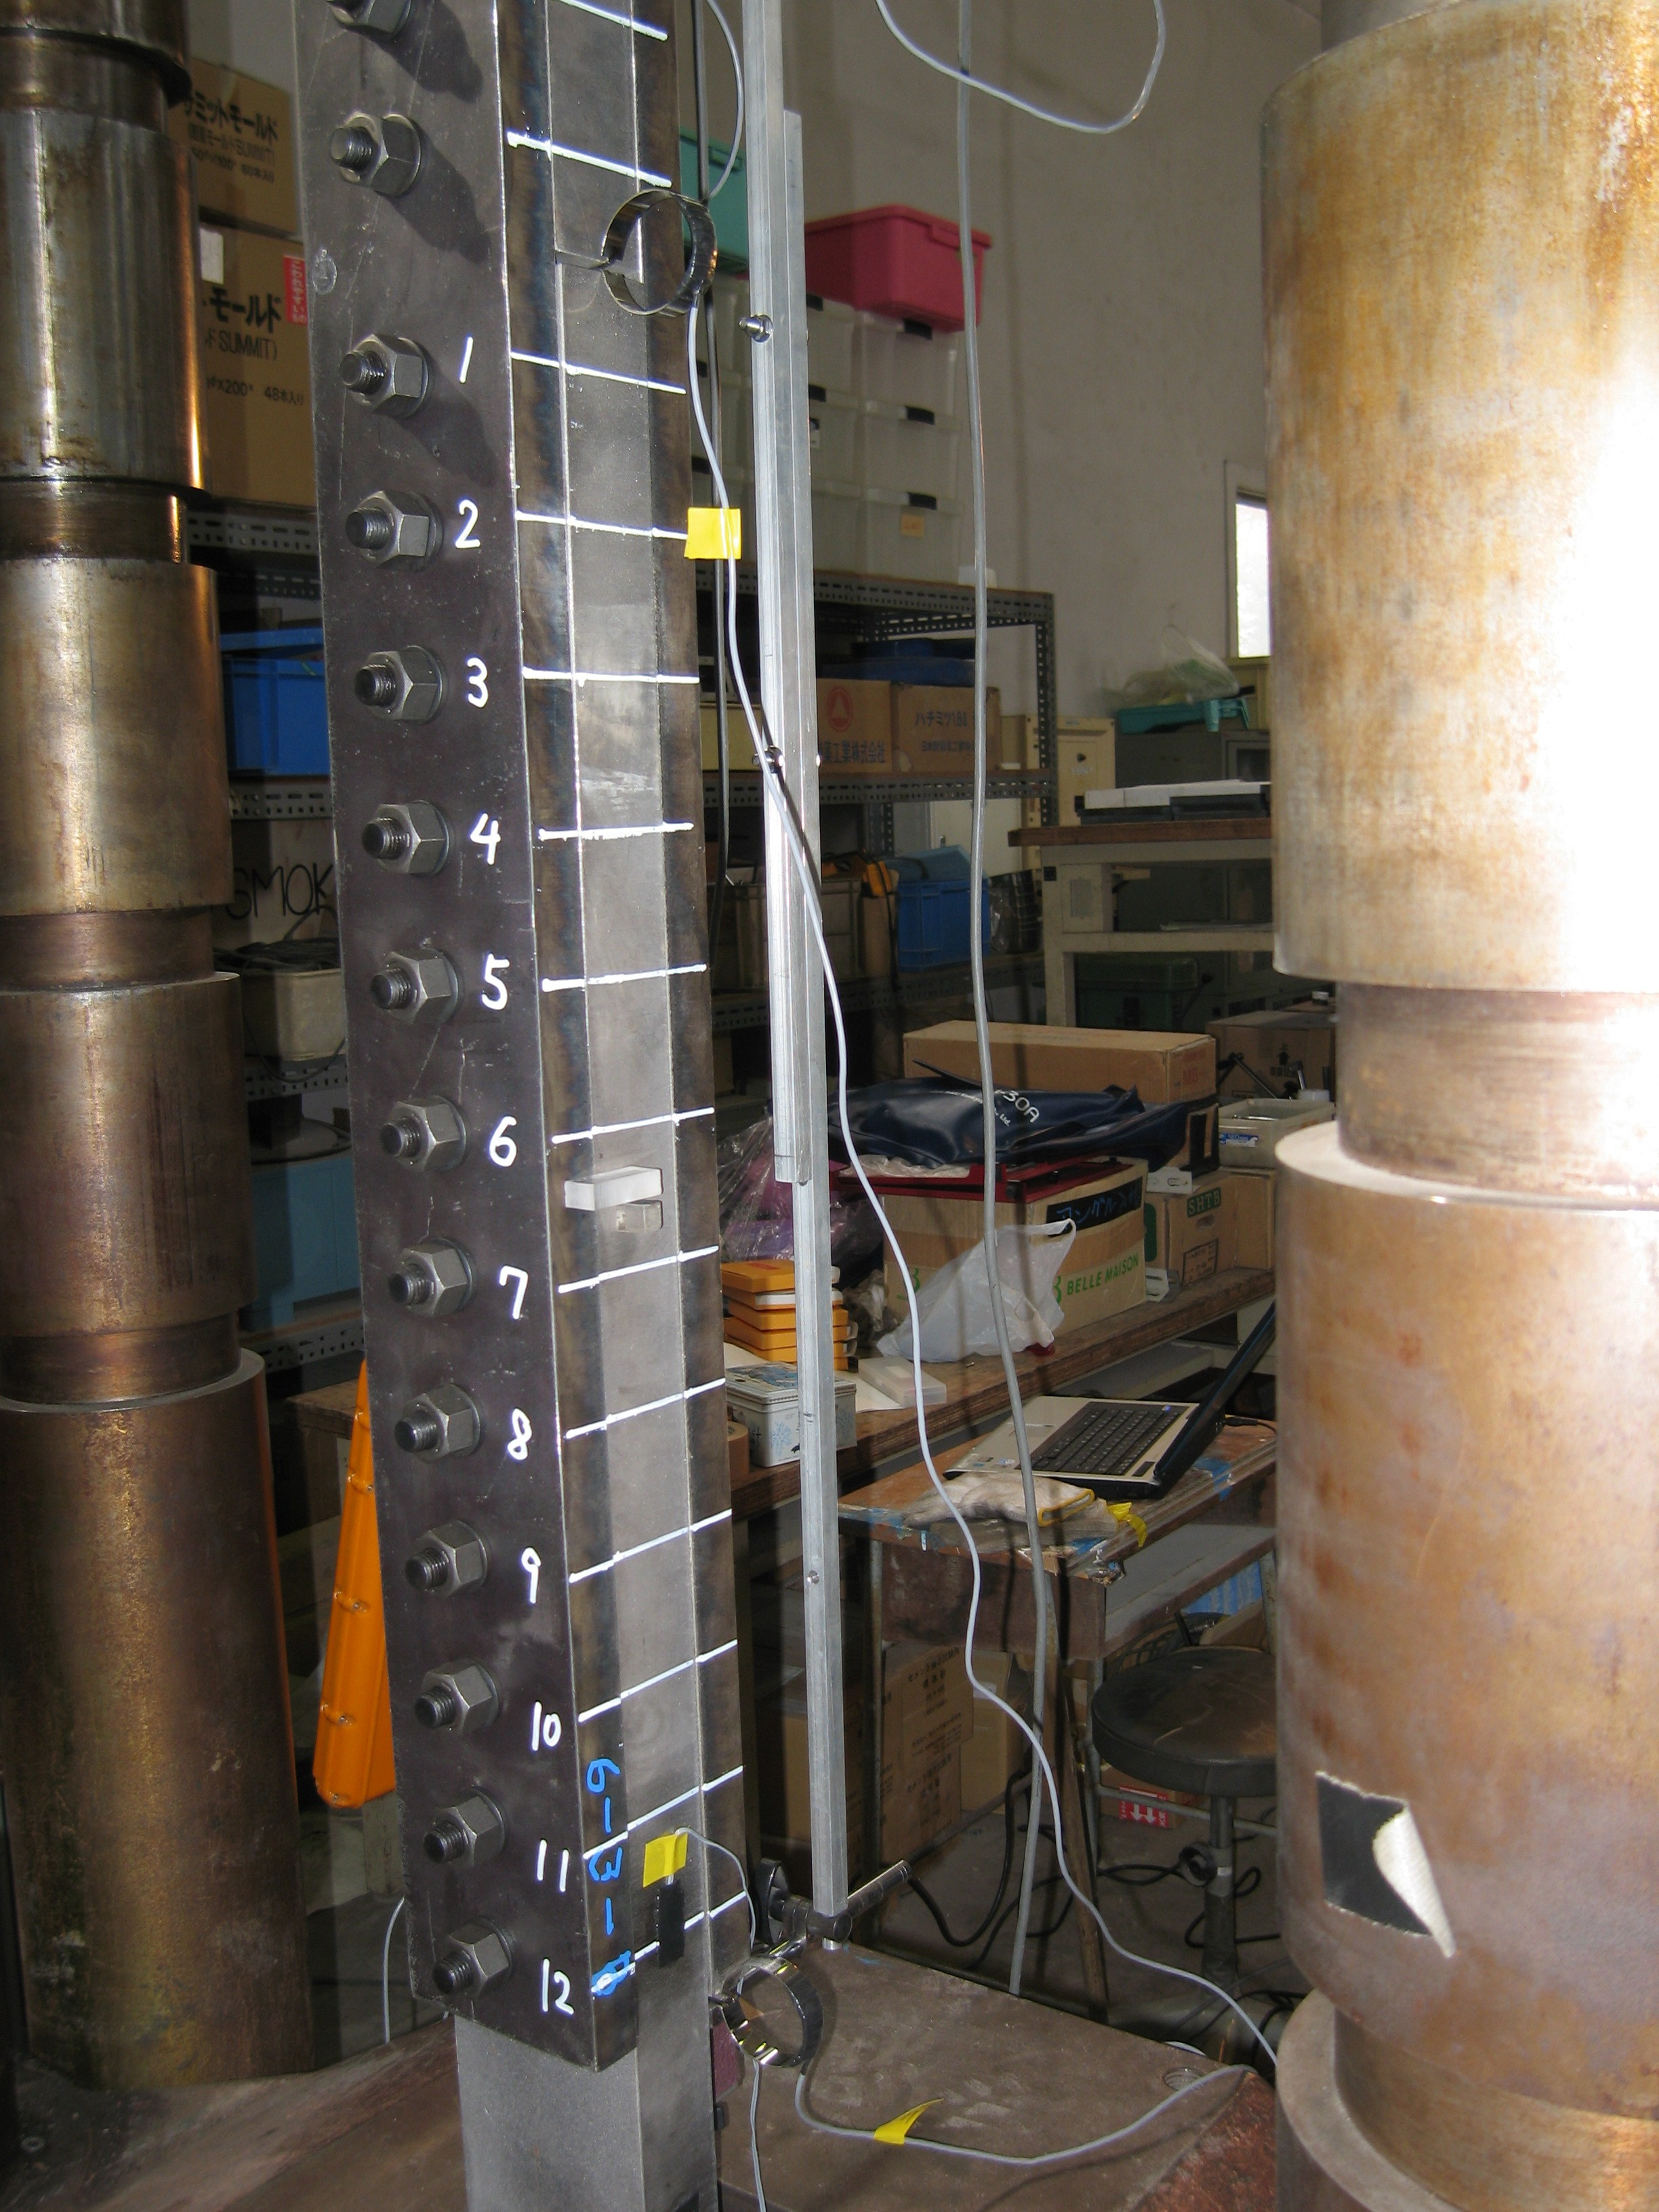
\includegraphics[width=\linewidth]{imgs/ch5/12rowtestpic.png}
        \caption{Setup of 12-row test specimen}
        \label{fig-testset}
    \end{subfigure}
    \hfill
    \begin{subfigure}[t]{0.55\textwidth}
        \centering
        \includegraphics[width=\linewidth]{imgs/ch5/validation.pdf}
        \caption{Validation of analysis model}
        \label{fig-validloadrd}
    \end{subfigure}
    \caption{Aging condition of rivet}
\end{figure}